%%%%%%%%%%%%%%%%%%%%%%%%%%%%%%%%%%%%%%%%%%%%%%%%%%%%%%%%%% Chap :
\chapter{Références}
\begin{itemize}
\item[Pepit.be :] Site web pepit, portails de jeux éducatifs
\item[Zoning :] Maquette d'une application ou site internet, sans design mais juste l'emplacement des éléments
\item[API :] Une interface de programmation (Application Programming Interface ou API) est une interface fournie par un programme informatique. Elle permet l'interaction des programmes les uns avec les autres, de manière analogue à une interface homme-machine, qui rend possible l'interaction entre un homme et une machine.
\end{itemize}


%%%%%%%%%%%%%%%%%%%%%%%%%%%%%%%%%%%%%%%%%%%%%%%%%%%%%%%%%% Chap :
%\chapter{Scripts de réunions}
%\section*{1\iere{} réunion (29/10/2012)}
%\label{reunion1}
%% les includes sont incomplets, il faut préciser la plage de page qu'on importe
%\includepdf{\dossierpdf reunion1_29_10_2012_debut_du_projet}
%\section*{2\ieme{} réunion (26/11/2012)}
%\includepdf{\dossierpdf reunion2_26_11_2012}
%\section*{3\ieme{} réunion (17/12/2012)}
%\includepdf{\dossierpdf reunion3_17_12_2012}


%%%%%%%%%%%%%%%%%%%%%%%%%%%%%%%%%%%%%%%%%%%%%%%%%%%%%%%%%% Chap :
\chapter{Architecture}
\label{annexe_architecture}
\includepdf[page=1-3]{\dossierpdf scenario}


%%%%%%%%%%%%%%%%%%%%%%%%%%%%%%%%%%%%%%%%%%%%%%%%%%%%%%%%%% Chap :
\chapter{Maquettes}
\section*{Maquette - Page d'accueil}
\begin{figure}[H]
\begin{center}
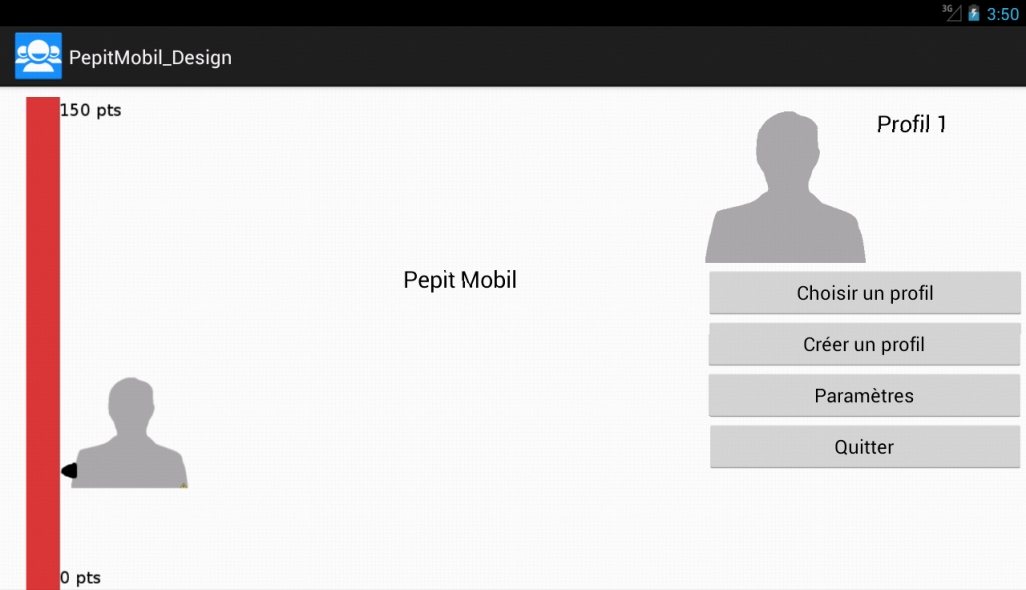
\includegraphics[width=15cm]{images/maquettes_homePage}
\end{center}
\caption{Pepit Mobil - Page d'accueil}
\label{Pepit Mobil - Page d'accueil}
\end{figure}

\section*{Maquette - Exercices}
\begin{figure}[H]
\begin{center}
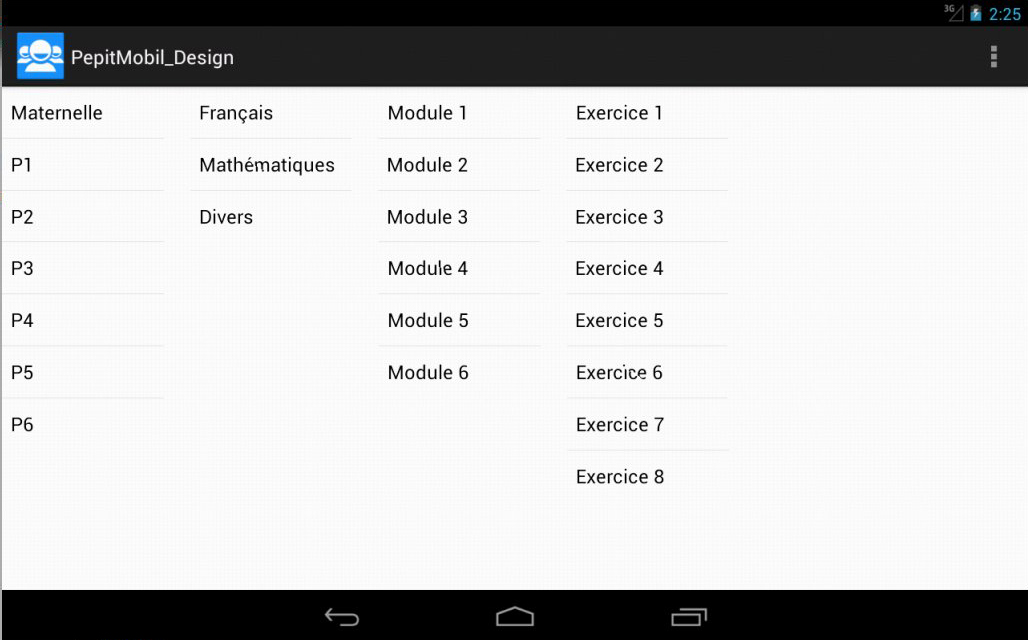
\includegraphics[width=15cm]{images/maquettes_exercices}
\end{center}
\caption{Pepit Mobil - Page exercices}
\label{Pepit Mobil - Page exercices}
\end{figure}

\section*{Maquette - Création de profil}
\begin{figure}[H]
\begin{center}
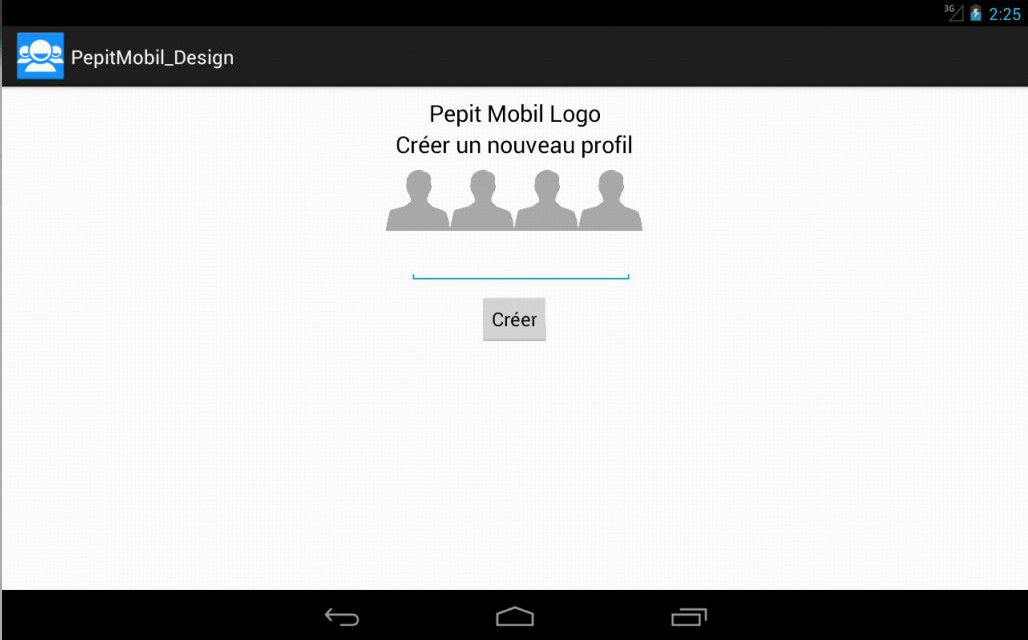
\includegraphics[width=15cm]{images/maquettes_creer_user}
\end{center}
\caption{Pepit Mobil - Page de création de profil}
\label{Pepit Mobil - Page de création de profil}
\end{figure}